\section{Case Studies}

We now sketch some examples of data analytics tasks that Meteor will provide support for. 

\subsection{Case Study: Top-K}

A top-K query is a common analytic query. For example, a cellular network operator may be interested in finding out the top-K applications users access on their mobile phones. Similarly, a search engine or CDN analyst will be interested in determining the top-K most visited URLs. 
A centralized algorithm for a top-K query will have to transfer all data to a central processing location and then aggregate, requiring a huge amount of bandwidth. For example, consider a network of 1000 cell towers, each connected to 50 mobile devices and generating a record for each device every two seconds. Each record has 200 fields, each field an integer value. The amount of data generated each minute over the network is therefore (1000 x 50 x 30 x 200 x 32) = 10 Gbits. Due to the sheer amount of data needed to be processed, it is much more preferable to process the data locally and do the aggregation only at the end. We plan to provide a top-k operator on top of Spark that implements the multi-round filtering approximate algorithm described in \cite{topk}.

\paragraph{The impact of sampling on Top-K queries.} As part of our case study, we wanted to evaluate the quality degradation on the output of a top-k query where sampling is performed to the input data set. Sampling can be used to reduce the input data set size. Thus, it can be used to reduce job completion time as well as the bandwidth requirements between nodes. 

Our experimental setup for this small study is the following: we execute a top K word-count MapReduce query on Spark without altering the input data set, and vary the top-K words that get reported for K ranging from 10 to 10000. We then run the same queries by reducing the size of the input data set by randomly sampling from the input data set. We then evaluate the error on the top-K word-count results when different sampling rates are applied. The sampling rates in our experiment range from 50\% down to 0.01\%. The error is derived from the percentage of the top-K words that appear in the ground truth query result (unaltered input data set). The results are summarized in figure \ref{fig:topk}.

\begin{figure}[ht]
    \centering
    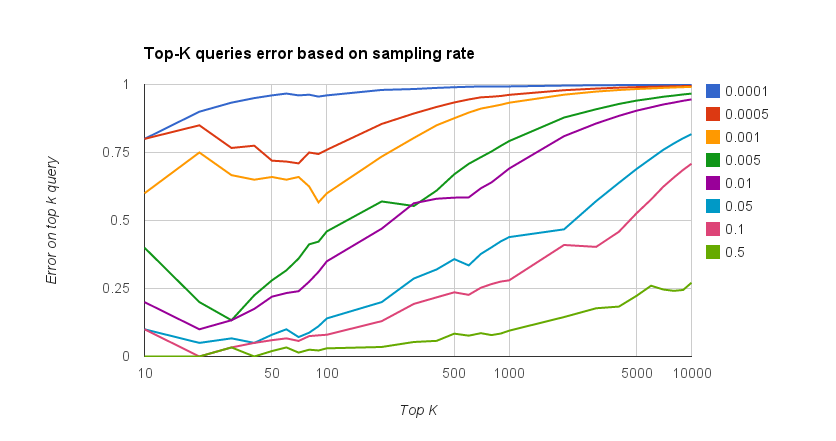
\includegraphics[width=5in]{figs/topk_sampling.png}
    \caption{The impact of sampling on Top-K query}
    \label{fig:topk}
\end{figure}

We observe that applying sampling on the input data set at a rate of 5\% and above introduces less than 10\% error on top-k queries where k is 50 or less. Reducing the sampling rate to 1\% will introduce less than 10\% error on top-k queries where k is 20 or less. For sampling rates below 1\%, we observe that the amount of error that gets introduced is too large for any value of k. 

We wish to evaluate the impact of sampling on job completion time and bandwidth requirements in a future study. We hope to find a practical use for sampling on our topologically-aware Spark system.

\subsection{Case Study: PageRank}

The PageRank algorithm is the cornerstone of Google's search technology. It is used to rank the many trillions of URLs by importance. PageRank iteratively updates a rank for each webpage by adding up contributions from each page that links to it. On each iteration, the contribution of each page to its neighbors is r/n, where r is its rank, and n is the number of neighbors.
PageRank is an iterative algorithm as opposed to top-K, which is a one-time query. The most bandwidth-hungry stage during a MapReduce implementation of PageRank is the reduce step that aggregates the parent URL for a URL key to compute its rank. We plan to evaluate an approximation where this global reduce step is delayed and done locally instead. 

